\chapter{Relacje porządku: od porównywania do kresów}\label{ch:orders}

\section{Dlaczego porządek to nie zawsze ustawienie w jednym szeregu?}
W zbiorze liczb rzeczywistych możemy porównać każdą parę liczb:
jedna jest mniejsza lub równa drugiej. Na zbiorze podzbiorów
ustalonego zbioru sytuacja jest inna. Dla $A=\{1\}$ i $B=\{2\}$
nie zachodzi ani $A\subseteq B$, ani $B\subseteq A$.
Mimo to zawieranie jest sensownym sposobem porządkowania podzbiorów.
Podobnie dwie różne liczby dodatnie nie zawsze dzielą się nawzajem,
a mimo to podzielność wyraża relację „bycia prostszym czynnikiem”.

Relacja równoważności z rozdziału~\ref{ch:equivalence} mówiła,
które obiekty uznajemy za nierozróżnialne. Relacja porządku
mówi, które obiekty można porównać i co z takiego porównania wynika.
W pierwszej kolejności rozróżnimy \emph{preporządek}, \emph{porządek
częściowy} i \emph{porządek liniowy}.

\begin{definicja}[Preporządek i porządek częściowy]\label{def:partial-order}
Niech $P$ będzie zbiorem, a $\preceq\subseteq P\times P$
relacją. Nazywamy ją \emph{preporządkiem}, jeśli jest zwrotna
i przechodnia. Nazywamy ją \emph{porządkiem częściowym}, jeśli
jest zwrotna, antysymetryczna i przechodnia.
Parę $(P,\preceq)$, w której $\preceq$ jest porządkiem
częściowym, nazywamy \emph{zbiorem częściowo uporządkowanym}.
Dwa elementy $a,b\in P$ są \emph{porównywalne}, jeśli
$a\preceq b$ lub $b\preceq a$. W przeciwnym razie są
\emph{nieporównywalne}.
\end{definicja}

\begin{przyklad}[Zawieranie podzbiorów]\label{ex:order-powerset}
Niech $X$ będzie zbiorem. Na $\mathcal P(X)$ relacja
$A\preceq B\iff A\subseteq B$
jest porządkiem częściowym: zwrotność zawierania wynika
z implikacji $x\in A\Rightarrow x\in A$, przechodniość
z dwóch kolejnych zawierań $A\subseteq B\subseteq C$,
a antysymetria z kryterium dwóch zawierań
(Twierdzenie~\ref{thm:two-inclusions}).
Dla $X=\{1,2\}$ podzbiory $\{1\}$ i $\{2\}$ są
nieporównywalne, ale obydwa leżą między $\varnothing$ i $X$.
\end{przyklad}

\begin{przyklad}[Podzielność wymaga wyboru zbioru podstawowego]
Na $\N_{>0}$ relacja $a\preceq b\iff a\mid b$ jest
zwrotna, gdyż $a=a\cdot1$. Jest przechodnia: z
$b=ak$ i $c=b\ell$ wynika $c=a(k\ell)$.
Jest też antysymetryczna: jeśli $b=ak$ i $a=b\ell$,
gdzie $a,b,k,\ell$ są dodatnimi liczbami całkowitymi, to
$a=a(k\ell)$, skąd $k\ell=1$, więc $k=\ell=1$ i $a=b$.
Na $\Z\setminus\{0\}$ podzielność \emph{nie} jest
antysymetryczna: $2\mid -2$ oraz $-2\mid2$, lecz $2\ne-2$.
\end{przyklad}

\begin{przyklad}[Preporządek, który nie jest porządkiem]
Na $\Z$ rozważmy $a\preceq b\iff |a|\le |b|$.
Zwrotność i przechodniość wynikają z własności porządku
liczb nieujemnych. Jednak $2\preceq -2$ i
$-2\preceq2$, a $2\ne-2$. Brakuje antysymetrii.
To pokazuje, dlaczego sama zwrotność i przechodniość
nie wystarczają do uzyskania porządku częściowego.
\end{przyklad}

\section{Porządki ostre, liniowe i przechodzenie od jednego do drugiego}
\label{sec:order-strict}
\begin{definicja}[Porządek ostry i porządek liniowy]\label{def:strict-total}
Relację $\prec$ na zbiorze $P$ nazywamy \emph{ostrym porządkiem
częściowym}, jeśli jest przeciwzwrotna i przechodnia.
Porządek częściowy $\preceq$ jest \emph{liniowy} (całkowity),
jeśli dla każdych $a,b\in P$ zachodzi $a\preceq b$ lub
$b\preceq a$. Ostry porządek jest \emph{ostrym porządkiem
liniowym}, jeżeli dla każdych różnych $a,b\in P$ zachodzi
$a\prec b$ lub $b\prec a$.
\end{definicja}

\begin{twierdzenie}[Przejście między porządkiem ostrym i nieostrym]
\label{thm:order-strict-correspondence}
Niech $P$ będzie zbiorem.
\begin{enumerate}[label=(\roman*)]
\item Jeżeli $\preceq$ jest porządkiem częściowym na $P$,
to relacja $\prec$ na $P$ określona dla $a,b\in P$ wzorem
$a\prec b\iff(a\preceq b\text{ i }a\ne b)$ jest ostrym
porządkiem częściowym.
\item Jeżeli $\prec$ jest ostrym porządkiem częściowym na $P$,
to relacja $\preceq$ na $P$ określona dla $a,b\in P$ wzorem
$a\preceq b\iff(a\prec b\text{ lub }a=b)$
jest porządkiem częściowym.
\item Obie konstrukcje są wzajemnie odwrotne i zachowują
liniowość.
\end{enumerate}
\end{twierdzenie}
\begin{proof}
(i) Ponieważ $a\ne a$ jest fałszem, żadne $a$ nie
spełnia $a\prec a$. Dla przechodniości załóżmy
$a\prec b$ i $b\prec c$. Z definicji mamy
$a\preceq b$ i $b\preceq c$, więc z przechodniości
$a\preceq c$. Gdyby $a=c$, to równocześnie zachodziłyby
$a\preceq b$ i $b\preceq a$. Antysymetria dawałaby
$a=b$, sprzecznie z $a\prec b$. Zatem $a\ne c$, a więc
$a\prec c$.

(ii) Nowa relacja jest zwrotna, bo $a=a$. Jeśli
$a\preceq b$ i $b\preceq a$, to albo $a=b$, albo
$a\prec b$ i $b\prec a$ (w przypadkach mieszanych
równość też dałaby $a=b$). Druga możliwość jest niemożliwa:
z przechodniości $a\prec a$, wbrew przeciwzwrotności.
Mamy zatem antysymetrię. Jeśli $a\preceq b$ i
$b\preceq c$, rozpatrujemy, czy każda z tych dwóch
relacji pochodzi z równości czy z $\prec$. Jeśli którakolwiek
jest równością, wynik $a\preceq c$ otrzymujemy bezpośrednio
z drugiej. Jeśli obie są ostre, daje go przechodniość $\prec$.

(iii) W pierwszej konstrukcji usuwamy dokładnie pary
$(a,a)$, a w drugiej dodajemy je z powrotem. Porządek ostry
nie zawiera par przekątnych, a porządek częściowy zawiera
wszystkie, więc odzyskujemy odpowiednio pierwotną relację.
Porównywalność różnych elementów jest niezmieniona;
dlatego liniowość obu wersji jest równoważna.
\end{proof}

\begin{przyklad}[Uwaga o słowie „ostry”]
Relacja $<$ na $\R$ jest ostrym porządkiem liniowym.
Dla dowolnego zbioru $X$ relacja właściwego zawierania
$\subsetneq$ na $\mathcal P(X)$ jest ostrym porządkiem częściowym,
ale gdy $X$ ma co najmniej dwa różne elementy,
nie jest liniowa: singletony tych elementów są
nieporównywalne. Ostrość i liniowość są niezależnymi cechami.
\end{przyklad}

\section{Łańcuchy, antyłańcuchy i diagramy Hassego}
\label{sec:order-hasse}
\begin{definicja}[Łańcuch i antyłańcuch]\label{def:chain-antichain}
Niech $(P,\preceq)$ będzie zbiorem częściowo uporządkowanym.
Podzbiór $C\subseteq P$ nazywamy \emph{łańcuchem}, jeśli
dowolne dwa elementy $C$ są porównywalne.
Podzbiór $D\subseteq P$ nazywamy \emph{antyłańcuchem}, jeśli
żadne dwa \emph{różne} elementy $D$ nie są porównywalne.
\end{definicja}

\begin{przyklad}[Podzbiory zbioru trójelementowego]
Na $\mathcal P(\{1,2,3\})$ rozważmy rodzinę
$\mathcal C=\{\varnothing,\{1\},\{1,2\},\{1,2,3\}\}$.
Jest ona łańcuchem, gdyż
$\varnothing\subsetneq\{1\}\subsetneq\{1,2\}\subsetneq\{1,2,3\}$.
Z kolei
$\{\{1\},\{2\},\{3\}\}$ jest antyłańcuchem:
żaden z trzech jednoelementowych zbiorów nie jest
podzbiorem innego. Te same elementy mogą brać udział
w różnych łańcuchach; łańcuch nie musi być maksymalny.
\end{przyklad}

\begin{definicja}[Relacja pokrywania]
W zbiorze częściowo uporządkowanym $(P,\preceq)$ oznaczmy
przez $a\prec b$ warunek $a\preceq b$ i $a\ne b$.
Mówimy, że $b$ \emph{pokrywa} $a$, i piszemy $a\lessdot b$, jeśli
$a\prec b$ oraz nie istnieje $c\in P$ takie, że
$a\prec c\prec b$.
Dla skończonego porządku \emph{diagram Hassego} ma po
jednym wierzchołku na element zbioru i krawędź prowadzącą
w górę od $a$ do $b$ dokładnie wtedy, gdy $a\lessdot b$.
Pomijamy pętle i krawędzie wynikające z przechodniości.
\end{definicja}

\begin{center}
\begin{tikzpicture}[scale=.85, every node/.style={font=\small}]
\node (e) at (0,0) {$\varnothing$};
\node (a) at (-1.4,1.5) {$\{1\}$};
\node (b) at (1.4,1.5) {$\{2\}$};
\node (t) at (0,3.0) {$\{1,2\}$};
\draw[thick] (e)--(a)--(t)--(b)--(e);
\node[font=\small,align=left,anchor=west] at (2.3,1.5)
{Brak krawędzi między\\$\{1\}$ i $\{2\}$: są\\nieporównywalne.};
\end{tikzpicture}

{\small Diagram Hassego porządku $(\mathcal P(\{1,2\}),\subseteq)$.}
\end{center}

\begin{uwaga}[Dlaczego na rysunku nie ma strzałek?]
Na diagramie Hassego umownie czytamy krawędzie od dołu do góry.
Na przykład $\varnothing\subseteq\{1,2\}$ odczytujemy
z dwukrawędziowej drogi przechodzącej przez $\{1\}$,
chociaż nie narysowano osobnej krawędzi od dolnego do górnego
wierzchołka. Dla skończonego porządku relację wyznaczają
osiągalność po krawędziach i równość elementów.
\end{uwaga}


\begin{przyklad}[Dwa elementy minimalne i brak najmniejszego]
Niech zbiór $P=\{a,b,c\}$ ma tylko porównania
$a\le c$, $b\le c$ oraz porównania wynikające ze zwrotności.
Elementy $a$ i $b$ są minimalne: nie mają elementów ściśle mniejszych.
Nie ma jednak elementu najmniejszego, bo $a\not\le b$ i $b\not\le a$.
W porządku liniowym taka sytuacja nie jest możliwa, ponieważ
dowolne dwa elementy można porównać.
\end{przyklad}

\section{Elementy najmniejsze, minimalne i ich odpowiedniki}
\label{sec:order-minmax}
\begin{definicja}[Minimum, maksimum, elementy minimalne i maksymalne]
\label{def:order-extrema}
Niech $(P,\preceq)$ będzie zbiorem częściowo uporządkowanym,
a $A\subseteq P$ podzbiorem. W poniższych warunkach
$a\prec b$ oznacza $a\preceq b$ i $a\ne b$.
\begin{enumerate}[label=(\roman*)]
\item $m\in A$ jest \emph{elementem najmniejszym} $A$,
jeśli $m\preceq a$ dla każdego $a\in A$.
\item $M\in A$ jest \emph{elementem największym} $A$,
jeśli $a\preceq M$ dla każdego $a\in A$.
\item $m\in A$ jest \emph{elementem minimalnym} $A$,
jeśli nie istnieje $a\in A$ z $a\prec m$.
\item $M\in A$ jest \emph{elementem maksymalnym} $A$,
jeśli nie istnieje $a\in A$ z $M\prec a$.
\end{enumerate}
Porządki w definicjach są ograniczeniami porządku z $P$ do $A$.
\end{definicja}

\begin{twierdzenie}[Jedyność elementów najmniejszych i największych]
\label{thm:order-least-unique}
W zbiorze częściowo uporządkowanym $(P,\preceq)$ każdy
podzbiór $A\subseteq P$ ma co najwyżej jeden element
najmniejszy i co najwyżej jeden element największy.
Każdy element najmniejszy jest minimalny, a każdy
największy jest maksymalny.
\end{twierdzenie}
\begin{proof}
Niech $m_1,m_2$ będą elementami najmniejszymi $A$.
Z definicji $m_1\preceq m_2$ i $m_2\preceq m_1$.
Antysymetria daje $m_1=m_2$. Podobnie, jeśli
$M_1,M_2$ są największe, to $M_1\preceq M_2$ i
$M_2\preceq M_1$, więc $M_1=M_2$.

Jeżeli $m$ jest najmniejszy, to dla każdego $a\in A$
zachodzi $m\preceq a$. Gdyby istniał $a\in A$ z
$a\prec m$, mielibyśmy także $a\preceq m$ i $a\ne m$,
co wraz z $m\preceq a$ przeczyłoby antysymetrii.
Zatem taki $a$ nie istnieje i $m$ jest minimalny.
Jeżeli zaś $M$ jest największy, to każdy $a\in A$ spełnia
$a\preceq M$. Gdyby istniał $b\in A$ z $M\prec b$,
mielibyśmy $M\preceq b$ i $M\ne b$. Ponieważ $M$ jest największy,
mamy także $b\preceq M$. Antysymetria wymusiłaby $b=M$,
wbrew nierówności. Zatem $M$ jest maksymalny.
\end{proof}

\begin{przyklad}[Dwa różne elementy minimalne]
Niech $P=\mathcal P(\{1,2\})$ z porządkiem zawierania,
a $A=\{\{1\},\{2\}\}$. Oba elementy $A$ są minimalne:
w $A$ nie ma od nich mniejszych elementów. Żaden nie jest
jednak najmniejszy, gdyż $\{1\}\nsubseteq\{2\}$
i $\{2\}\nsubseteq\{1\}$. Analogicznie oba są
maksymalne, ale nie ma elementu największego.
Jest to podstawowy kontrprzykład do mylenia minimum z
minimalnością.
\end{przyklad}

\begin{twierdzenie}[Istnienie ekstremów w skończonym porządku]
\label{thm:finite-poset-extrema}
Niech $(P,\preceq)$ będzie zbiorem częściowo
uporządkowanym, a $A\subseteq P$ niepustym skończonym
podzbiorem. Wtedy $A$ ma element minimalny i element
maksymalny. Niekoniecznie ma element najmniejszy lub
największy.
\end{twierdzenie}
\begin{proof}
Wybierzmy $a_0\in A$; można to zrobić, ponieważ $A$
jest niepusty. Jeśli $a_0$ jest minimalny, mamy tezę.
W przeciwnym razie istnieje $a_1\in A$ z
$a_1\prec a_0$. Jeżeli $a_1$ nie jest minimalny,
znajdujemy $a_2\in A$ z $a_2\prec a_1$ itd.
W każdym kroku otrzymujemy element różny od wszystkich
wcześniejszych: gdyby $a_j=a_i$ dla $j>i$, to z
przechodniości wynikłoby $a_i\prec a_i$, sprzecznie
z przeciwzwrotnością ostrego porządku
(Twierdzenie~\ref{thm:order-strict-correspondence}).
Ponieważ $A$ jest skończony, nie możemy wytworzyć
dowolnie długiego ciągu parami różnych elementów $A$.
Proces musi zakończyć się na elemencie minimalnym.

Aby uzyskać element maksymalny, powtarzamy argument,
zastępując każdy krok $a_{j+1}\prec a_j$ krokiem
$a_j\prec a_{j+1}$. Ponownie skończoność wymusza
zakończenie. Przykład z dwoma singletonami powyżej
pokazuje, że minimum i maksimum nie muszą istnieć.
\end{proof}


\begin{twierdzenie}[Odczytywanie porządku z diagramu Hassego]
\label{thm:hasse-paths-xliii}
Niech $(P,\preceq)$ będzie \emph{skończonym} zbiorem
częściowo uporządkowanym. Dla $x,y\in P$ piszemy $x\prec y$,
gdy $x\preceq y$ i $x\ne y$, oraz $x\lessdot y$,
gdy $x\prec y$ i nie istnieje $z\in P$ z $x\prec z\prec y$.
Dla różnych $a,b\in P$ zachodzi $a\prec b$
wtedy i tylko wtedy, gdy istnieją
$a=x_0,x_1,\ldots,x_k=b$ z $k\ge1$ i
$x_{j-1}\lessdot x_j$ dla każdego $j=1,\ldots,k$.
Zatem porządek można odtworzyć z diagramu Hassego,
dodając równość elementów i przechodniość wzdłuż
rosnących dróg.
\end{twierdzenie}
\begin{proof}
Jeżeli istnieje taka droga, każda krawędź pokrywania
spełnia $x_{j-1}\prec x_j$. Przechodniość daje
$a\prec b$ (dla $k=1$ jest to pierwsza krawędź).

W przeciwnym kierunku załóżmy $a\prec b$.
Rozważmy skończony, niepusty zbiór
$S=\{x\in P:a\prec x\preceq b\}$; należy do niego $b$.
Na mocy Twierdzenia~\ref{thm:finite-poset-extrema}
$S$ ma element minimalny $x_1$. Mamy $a\prec x_1$.
Gdyby istniało $z$ z $a\prec z\prec x_1$, to
$z\preceq x_1\preceq b$ i $z\in S$,
co przeczyłoby minimalności $x_1$. Zatem $a\lessdot x_1$.
Jeśli $x_1=b$, kończymy. W przeciwnym razie stosujemy
identyczną konstrukcję do pary $x_1\prec b$.
Każdy krok daje większy element $x_j\preceq b$;
żaden nie może powtórzyć wcześniejszego, bo wówczas
z przechodniości wynikałoby $x_j\prec x_j$.
Skończoność $P$ wymusza zakończenie i osiągnięcie $b$.
\end{proof}
\begin{przyklad}[Dlaczego skończoność jest istotna]
\label{ex:hasse-infinite-caution-xliii}
Na $(\Q,\le)$ nie istnieje żadna para $a\lessdot b$:
jeśli $a<b$, liczba $c=(a+b)/2$ jest wymierna i
spełnia $a<c<b$. Diagram z samymi krawędziami
pokrywania nie miałby więc żadnej krawędzi, choć
wiele liczb jest porównywalnych. Odczytywanie porządku
z dróg diagramu Hassego bez założenia skończoności
jest w ogólności błędne.
\end{przyklad}


\begin{twierdzenie}[Jedyny element minimalny w skończonym porządku]
\label{thm:unique-minimal-finite-xliii}
Niech $(P,\preceq)$ będzie zbiorem częściowo uporządkowanym,
a $A\subseteq P$ niepustym, skończonym podzbiorem.
Wtedy $A$ ma dokładnie jeden element minimalny wtedy i tylko
wtedy, gdy ma element najmniejszy.
Analogicznie $A$ ma dokładnie jeden element maksymalny
wtedy i tylko wtedy, gdy ma element największy.
\end{twierdzenie}
\begin{proof}
Jeżeli $m$ jest elementem najmniejszym $A$, to jest
minimalny na mocy Twierdzenia~\ref{thm:order-least-unique}.
Gdyby $u\ne m$ był innym elementem minimalnym, to
$m\preceq u$ i $m\ne u$, czyli $m\prec u$,
sprzecznie z minimalnością $u$. Zatem $m$ jest jedynym
minimalnym elementem.

Odwrotnie, niech $m$ będzie jedynym minimalnym elementem $A$.
Wybierzmy dowolny $a\in A$. Zbiór
$D_a=\{x\in A:x\preceq a\}$ jest niepusty (zawiera $a$)
i skończony. Na mocy
Twierdzenia~\ref{thm:finite-poset-extrema} ma element
minimalny $u$. Gdyby istniał $v\in A$ z $v\prec u$,
to $v\preceq u\preceq a$, a więc $v\in D_a$;
byłaby to sprzeczność z minimalnością $u$ w $D_a$.
Zatem $u$ jest minimalny w całym $A$, czyli $u=m$.
Ponieważ $u\in D_a$, mamy $m\preceq a$. Element $a$
był dowolny, więc $m$ jest najmniejszy w $A$.
Dla elementów maksymalnych rozumowanie działa z odwróconym
kierunkiem porządku: w miejscu $D_a$ stosujemy
$\{x\in A:a\preceq x\}$.
\end{proof}

\begin{przyklad}[Jedyny element minimalny nie musi być najmniejszy]
\label{ex:unique-minimal-infinite-xliii}
Skończoności nie można usunąć z poprzedniego twierdzenia.
Niech $P=\{m\}\cup\{b_n:n\in\N\}$, przy czym
wszystkie oznaczenia są różnymi elementami.
Ustalmy zwrotne porównania oraz
$b_j\preceq b_i$ dokładnie wtedy, gdy $j\ge i$;
nie porównujemy $m$ z żadnym $b_i$.
Wtedy $P$ jest zbiorem częściowo uporządkowanym.
Element $m$ jest minimalny, bo nic nie leży ściśle
poniżej niego. Żaden $b_i$ nie jest minimalny, gdyż
$b_{i+1}\prec b_i$. Zatem $m$ jest \emph{jedynym}
elementem minimalnym, lecz nie jest elementem najmniejszym:
nie zachodzi $m\preceq b_0$.
W podzbiorze $\{b_n:n\in\N\}$ nie ma żadnego
elementu minimalnego. To właśnie umożliwia kontrprzykład.

\begin{center}
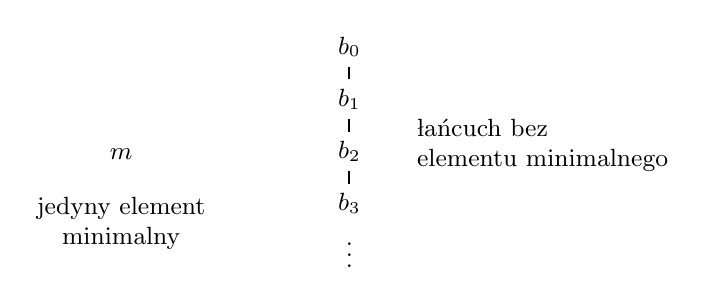
\begin{tikzpicture}[x=.92cm,y=.78cm, every node/.style={font=\small}]
 \node (m) at (-1.9,1.45) {$m$};
 \node (b0) at (1.25,3.2) {$b_0$};
 \node (b1) at (1.25,2.35) {$b_1$};
 \node (b2) at (1.25,1.50) {$b_2$};
 \node (b3) at (1.25,.65) {$b_3$};
 \draw[thick] (b0)--(b1)--(b2)--(b3);
 \node at (1.25,-.06) {$\vdots$};
 \node[anchor=north,align=center] at (-1.9,.92) {jedyny element\\minimalny};
 \node[anchor=west,align=left] at (2.05,1.6) {łańcuch bez\\elementu minimalnego};
\end{tikzpicture}

{\small Schemat nieskończonego porządku: $m$ jest nieporównywalny
z każdym $b_n$, a łańcuch po prawej biegnie w dół bez końca.}
\end{center}
\end{przyklad}

\section{Ograniczenia, kres dolny i kres górny}\label{sec:order-bounds}
\begin{definicja}[Ograniczenia i kresy]\label{def:bounds-sup-inf}
Niech $(P,\preceq)$ będzie zbiorem częściowo uporządkowanym,
a $A\subseteq P$.
Element $u\in P$ jest \emph{ograniczeniem górnym} $A$,
jeżeli $a\preceq u$ dla wszystkich $a\in A$.
Element $\ell\in P$ jest \emph{ograniczeniem dolnym} $A$,
jeżeli $\ell\preceq a$ dla wszystkich $a\in A$.

Jeśli zbiór wszystkich ograniczeń górnych $A$ ma element
najmniejszy, nazywamy go \emph{kresem górnym} $A$ i piszemy
$\sup_P A$. Jeśli zbiór wszystkich ograniczeń dolnych
ma element największy, nazywamy go \emph{kresem dolnym} $A$
i piszemy $\inf_P A$. Symbolu kresu używamy tylko, gdy
taki element istnieje w $P$.
\end{definicja}

\begin{uwaga}[Kres nie musi należeć do rozpatrywanego zbioru]
W $P=\R$ z naturalnym porządkiem zbiór
$A=(0,1)$ ma $\sup_{\R}A=1$ i $\inf_{\R}A=0$,
ale żaden z tych kresów nie należy do $A$.
W zbiorze liczb wymiernych $\Q$ zbiór
$B=\{q\in\Q:q\ge0,\ q^2<2\}$ nie ma kresu górnego
\emph{w $\Q$}: jedyny rzeczywisty kres to $\sqrt2$,
który nie należy do $\Q$. Stąd w definicji zawsze
wskazujemy, w jakim porządku szukamy kresu.
\end{uwaga}

\begin{twierdzenie}[Kryterium kresu górnego]\label{thm:sup-characterization}
Niech $(P,\preceq)$ będzie zbiorem częściowo uporządkowanym,
a $A\subseteq P$. Element $s\in P$ jest kresem górnym $A$
wtedy i tylko wtedy, gdy
\begin{enumerate}[label=(\roman*)]
\item dla każdego $a\in A$ zachodzi $a\preceq s$;
\item dla każdego $u\in P$, jeżeli $a\preceq u$ dla każdego
$a\in A$, to $s\preceq u$.
\end{enumerate}
Analogicznie $t\in P$ jest kresem dolnym $A$ wtedy
i tylko wtedy, gdy $t\preceq a$ dla wszystkich $a\in A$
oraz $\ell\preceq t$ dla każdego ograniczenia dolnego
$\ell$ zbioru $A$.
\end{twierdzenie}
\begin{proof}
Z definicji $s=\sup_P A$ znaczy, że jest
\emph{najmniejszym} elementem zbioru wszystkich ograniczeń
górnych. To dokładnie oznacza, że sam jest ograniczeniem
górnym (warunek (i)) oraz że leży poniżej każdego innego
ograniczenia górnego (warunek (ii)). Każdy z tych dwóch
warunków jest konieczny, a ich koniunkcja wystarcza.
Dla kresu dolnego odwracamy kierunek relacji i powtarzamy
ten sam argument. Jedyność kresów wynika z
Twierdzenia~\ref{thm:order-least-unique} zastosowanego
do zbiorów ograniczeń.
\end{proof}

\begin{przyklad}[Suma i przecięcie jako kresy]\label{ex:orders-sets-lattice}
Niech $X$ będzie zbiorem, a $A,B\subseteq X$. W porządku
$(\mathcal P(X),\subseteq)$ zachodzą równości
\[
 \sup_{\mathcal P(X)}\{A,B\}=A\cup B,\qquad
 \inf_{\mathcal P(X)}\{A,B\}=A\cap B.
\]
Istotnie, $A\subseteq A\cup B$ i $B\subseteq A\cup B$,
więc suma jest ograniczeniem górnym pary $\{A,B\}$.
Jeśli $U$ jest dowolnym ograniczeniem górnym, to
$A\subseteq U$ i $B\subseteq U$, z czego dla każdego
$x\in A\cup B$ wynika $x\in U$. A zatem
$A\cup B\subseteq U$, więc suma jest najmniejszym
ograniczeniem górnym. Dla przecięcia analogicznie:
$A\cap B$ zawiera się w obu zbiorach, a każdy
podzbiór zawarty jednocześnie w $A$ i $B$ zawiera się
w $A\cap B$.
\end{przyklad}

\begin{przyklad}[Największy wspólny dzielnik i najmniejsza wspólna wielokrotność]
Niech $a,b\in\N_{>0}$. W porządku podzielności na $\N_{>0}$
ograniczeniami
dolnymi pary $\{a,b\}$ są dokładnie wspólne dzielniki
$a,b$, a górnymi --- ich wspólne wielokrotności.
Kresem dolnym tej pary jest $\gcd(a,b)$, a górnym
$\operatorname{lcm}(a,b)$. Dla $a=12$, $b=18$
mamy $\inf\{12,18\}=6$ i $\sup\{12,18\}=36$
\emph{w porządku podzielności}, mimo że w zwykłym
porządku liczb naturalnych minimum tej pary to $12$,
a maksimum to $18$.
\end{przyklad}

\section{Kraty i działania kresowe}\label{sec:order-lattices}
\begin{definicja}[Krata]\label{def:lattice}
Zbiór częściowo uporządkowany $(L,\preceq)$ jest
\emph{kratą}, jeśli każda para $a,b\in L$ ma kres
dolny $a\wedge b$ i kres górny $a\vee b$ w $L$.
Krata jest \emph{zupełna}, jeśli \emph{każdy} podzbiór
$A\subseteq L$, także pusty, ma kres dolny i kres górny.
\end{definicja}

\begin{twierdzenie}[Pusta rodzina i krańcowe elementy kraty zupełnej]
\label{thm:complete-lattice-bottom-top-xliii}
Jeśli $(L,\preceq)$ jest kratą zupełną, to $L$ ma
jedyny element najmniejszy $0_L$ oraz jedyny element
największy $1_L$. Ponadto
$0_L=\sup_L\varnothing$ i $1_L=\inf_L\varnothing$.
Nie każda krata jest zupełna: nawet krata, w której istnieją
kresy wszystkich skończonych niepustych podzbiorów, może
nie mieć kresów pewnych podzbiorów nieskończonych.
\end{twierdzenie}
\begin{proof}
Z definicji zupełności istnieje $s=\sup_L\varnothing$.
Każdy element $u\in L$ jest ograniczeniem górnym pustego
zbioru, ponieważ nie ma elementu $a\in\varnothing$,
który mógłby naruszyć nierówność $a\preceq u$.
Skoro $s$ jest \emph{najmniejszym} z tych ograniczeń,
to $s\preceq u$ dla wszystkich $u\in L$. Jest więc
najmniejszy. Analogicznie każdy element $\ell\in L$
jest ograniczeniem dolnym pustego zbioru, a jego największe
ograniczenie dolne $t=\inf_L\varnothing$ spełnia
$\ell\preceq t$ dla każdego $\ell\in L$.
Jest więc największy. Oba elementy są jedyne dzięki
antysymetrii. Samo istnienie $s$ pokazuje, że krata
zupełna musi być niepusta.

Aby wykazać, że nie każda krata jest zupełna, rozważmy
$(\N,\le)$. Każda para liczb naturalnych ma minimum
i maksimum, lecz cały zbiór $\N$ nie ma ograniczenia
górnego w $\N$: dla każdego $u\in\N$ zachodzi
$u<u+1$. Zatem $\sup_{\N}\N$ nie istnieje.
\end{proof}
\begin{przyklad}[Krata, która nie jest zupełna]
\label{ex:lattice-not-complete-xliii}
Rozważmy $L=\N$ ze zwykłym porządkiem (z zerem).
Każda para liczb naturalnych ma minimum i maksimum,
więc $L$ jest kratą. Co więcej, każdy niepusty
skończony podzbiór ma minimum i maksimum. Jednak zbiór
$A=\N\subseteq L$ nie ma w $L$ żadnego ograniczenia
górnego: dla dowolnego $u\in\N$ liczba $u+1\in A$
jest większa niż $u$. W konsekwencji $\sup_L A$
nie istnieje i krata $L$ nie jest zupełna.
Dodatkowo $\inf_L\varnothing$ nie istnieje, bo
$\N$ nie ma elementu największego.
\end{przyklad}


\begin{twierdzenie}[Podstawowe prawa działań w kracie]\label{thm:lattice-laws}
Niech $(L,\preceq)$ będzie kratą. Dla wszystkich
$a,b,c\in L$ zachodzą
\begin{align*}
 a\wedge b&=b\wedge a,&a\vee b&=b\vee a,\\
 (a\wedge b)\wedge c&=a\wedge(b\wedge c),&
 (a\vee b)\vee c&=a\vee(b\vee c),\\
 a\wedge a&=a,&a\vee a&=a,\\
 a\wedge(a\vee b)&=a,&a\vee(a\wedge b)&=a.
\end{align*}
\end{twierdzenie}
\begin{proof}
Ponieważ zbiór $\{a,b\}$ nie zmienia się po zamianie
$a$ i $b$, jego kresy także się nie zmieniają.
To dowodzi przemienności obu działań.

Dla łączności $\wedge$ zauważmy, że
$(a\wedge b)\wedge c$ jest największym elementem
leżącym jednocześnie poniżej $a\wedge b$ i $c$.
Każdy taki element leży poniżej $a$, $b$ i $c$.
Odwrotnie, jeśli $x\preceq a,b,c$, to z definicji
$a\wedge b$ wynika $x\preceq a\wedge b$, a ponadto
$x\preceq c$; zatem $x\preceq(a\wedge b)\wedge c$.
Pokazuje to, że $(a\wedge b)\wedge c$ jest
największym wspólnym ograniczeniem dolnym trzech
elementów. Dokładnie ten sam argument, zaczynając
od pary $(b,c)$, pokazuje, że $a\wedge(b\wedge c)$
ma tę samą własność. Jedyność kresu daje równość.
Dla $\vee$ zamieniamy we wszystkich zdaniach
„poniżej” na „powyżej” i „największe ograniczenie dolne”
na „najmniejsze ograniczenie górne”.

Dla idempotentności obserwujemy, że $a$ jest zarazem
największym elementem poniżej $a,a$ i najmniejszym
powyżej $a,a$. Stąd $a\wedge a=a\vee a=a$.
Dla absorpcji: $a\preceq a\vee b$, więc $a$ jest
dolnym ograniczeniem pary $\{a,a\vee b\}$.
Każde dolne ograniczenie tej pary musi leżeć poniżej $a$,
zatem $a$ jest jej kresem dolnym, czyli
$a\wedge(a\vee b)=a$. Analogicznie
$a\wedge b\preceq a$ i każde ograniczenie górne
pary $\{a,a\wedge b\}$ leży powyżej $a$;
stąd $a\vee(a\wedge b)=a$.
\end{proof}

\begin{uwaga}[Nie każda krata jest rozdzielna]
Prawa absorpcji są prawdziwe w każdej kracie, ale
prawa rozdzielności nie muszą zachodzić. Istotnym
kontrprzykładem jest pięcioelementowa krata z trzema
wzajemnie nieporównywalnymi elementami $a,b,c$ między
najmniejszym $0$ a największym $1$.
W niej $b\vee c=1$, więc $a\wedge(b\vee c)=a$,
a jednocześnie $a\wedge b=a\wedge c=0$, zatem
$(a\wedge b)\vee(a\wedge c)=0\ne a$.
Nie wolno więc uogólniać praw rozdzielności sum i
przecięć zbiorów z rozdziału~\ref{ch:sets} na wszystkie kraty.
\end{uwaga}

\begin{center}
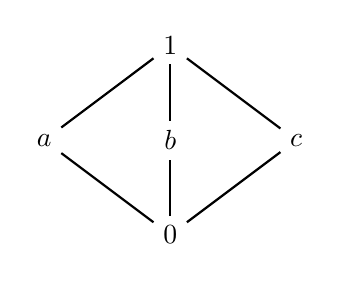
\begin{tikzpicture}[scale=.8]
 \node (z) at (0,0) {$0$}; \node (o) at (0,3) {$1$};
 \node (a) at (-2,1.5) {$a$};
 \node (b) at (0,1.5) {$b$};
 \node (c) at (2,1.5) {$c$};
 \foreach \x in {a,b,c} {\draw[thick] (z)--(\x)--(o);}
\end{tikzpicture}

{\small Krata $M_3$: trzy nieporównywalne elementy między $0$ i $1$.}
\end{center}

\begin{twierdzenie}[Krata podzbiorów jest zupełna]
\label{thm:powerset-complete-lattice}
Niech $X$ będzie dowolnym zbiorem. W porządku
$(\mathcal P(X),\subseteq)$ każda rodzina
$\mathcal A\subseteq\mathcal P(X)$ ma kresy
\[
 \sup\mathcal A=\bigcup_{A\in\mathcal A}A,
 \qquad \inf\mathcal A=\bigcap_{A\in\mathcal A}A,
\]
gdzie dla $\mathcal A=\varnothing$ przyjmujemy
$\bigcap_{A\in\mathcal A}A=X$. W szczególności
$(\mathcal P(X),\subseteq)$ jest kratą zupełną.
\end{twierdzenie}
\begin{proof}
Dla każdego $A\in\mathcal A$ mamy
$A\subseteq\bigcup_{B\in\mathcal A}B$, a jeżeli
$U\subseteq X$ zawiera każdy $A\in\mathcal A$, to
z definicji sumy zawiera także całą sumę. Suma jest więc
najmniejszym ograniczeniem górnym. Analogicznie
przecięcie zawiera się w każdym $A$, a każdy
$D\subseteq X$ zawarty w każdym $A$ zawiera się
w ich przecięciu, dlatego jest największym
ograniczeniem dolnym. Jeśli $\mathcal A$ jest pusta,
każdy podzbiór $X$ jest zarówno ograniczeniem górnym,
jak i dolnym pustej rodziny: najmniejszym w
$\mathcal P(X)$ jest $\varnothing$, największym $X$.
Z definicji sumy i pustego przecięcia wynika dokładnie
$\sup\varnothing=\varnothing$ i $\inf\varnothing=X$.
\end{proof}

\section{Porządki iloczynowe i leksykograficzne}\label{sec:order-products}
\begin{definicja}[Porządek współrzędny]
Niech $(P,\preceq_P)$ i $(Q,\preceq_Q)$ będą
zbiorami częściowo uporządkowanymi. Na $P\times Q$
określamy
\[
 (p,q)\preceq_\times(p',q')\iff
 p\preceq_P p'\ \text{oraz}\ q\preceq_Q q'.
\]
Nazywamy go \emph{porządkiem współrzędnym}.
\end{definicja}

\begin{twierdzenie}[Porządek współrzędny jest częściowy]
\label{thm:product-poset}
Niech $(P,\preceq_P)$ i $(Q,\preceq_Q)$ będą zbiorami
częściowo uporządkowanymi. Na $P\times Q$ określmy relację
$(p,q)\preceq_\times(p',q')$ wtedy i tylko wtedy, gdy
$p\preceq_P p'$ oraz $q\preceq_Q q'$.
Wtedy $\preceq_\times$ jest porządkiem częściowym na $P\times Q$.
\end{twierdzenie}
\begin{proof}
Dla $(p,q)$ zwrotność obu porządków daje
$p\preceq_P p$ i $q\preceq_Q q$,
czyli $(p,q)\preceq_\times(p,q)$.
Jeśli $(p,q)\preceq_\times(p',q')$ i odwrotnie,
to antysymetria na $P$ daje $p=p'$, a na $Q$ daje
$q=q'$. Z jednoznaczności współrzędnych par
(Twierdzenie~\ref{thm:kuratowski}) wynika
$(p,q)=(p',q')$. Jeśli mamy dwa kolejne porównania
$(p,q)\preceq_\times(p',q')$ oraz
$(p',q')\preceq_\times(p'',q'')$, to przechodniość
na $P$ daje $p\preceq_P p''$, a na $Q$ daje
$q\preceq_Q q''$, czyli zachodzi przechodniość na iloczynie.
\end{proof}

\begin{przyklad}[Nieporównywalność w produkcie]
Nawet gdy $P=Q=\R$ z porządkiem liniowym,
porządek współrzędny na $\R^2$ nie jest liniowy:
$(0,1)$ i $(1,0)$ są nieporównywalne.
Pierwszy punkt ma mniejszą pierwszą współrzędną,
ale większą drugą; żaden nie dominuje drugiego
w obu współrzędnych.
\end{przyklad}

\begin{definicja}[Porządek leksykograficzny]
Niech $(P,\preceq_P)$ i $(Q,\preceq_Q)$ będą
zbiorami liniowo uporządkowanymi, a $\prec_P,\prec_Q$
ich ostrymi odpowiednikami. Na $P\times Q$ ustalamy
\[
 (p,q)\preceq_{\rm lex}(p',q')\iff
 (p\prec_P p')\ \text{lub}\ (p=p'\text{ i }q\preceq_Q q').
\]
Najpierw porównujemy pierwszą współrzędną, a dopiero
przy remisie drugą.
\end{definicja}

\begin{twierdzenie}[Porządek leksykograficzny jest liniowy]
\label{thm:lex-order}
Niech $(P,\preceq_P)$ i $(Q,\preceq_Q)$ będą zbiorami
liniowo uporządkowanymi, a $p\prec_P p'$ niech oznacza
$p\preceq_P p'$ i $p\ne p'$. Na $P\times Q$ określmy
$(p,q)\preceq_{\rm lex}(p',q')$ wtedy i tylko wtedy, gdy
$p\prec_P p'$ lub ($p=p'$ i $q\preceq_Q q'$).
Wtedy $\preceq_{\rm lex}$ jest porządkiem liniowym na $P\times Q$.
\end{twierdzenie}
\begin{proof}
Zwrotność: $p=p$ i $q\preceq_Q q$.
Dla antysymetrii załóżmy oba porównania w przeciwnych
kierunkach. Jeżeli $p\prec_P p'$, to porównanie odwrotne
nie może zachodzić: wymagałoby $p'\prec_P p$ lub
$p'=p$, a obie możliwości są sprzeczne z asymetrią
$\prec_P$. Podobnie nie może zachodzić $p'\prec_P p$.
Pozostaje więc $p=p'$, a z obu porównań dostajemy
$q\preceq_Q q'$ i $q'\preceq_Q q$. Antysymetria
daje $q=q'$, zatem równość par.

Dla przechodniości załóżmy
$(p,q)\preceq_{\rm lex}(p',q')$ i
$(p',q')\preceq_{\rm lex}(p'',q'')$.
Jeśli $p\prec_P p'$, to z $p'\preceq_P p''$
i przechodniości otrzymujemy $p\preceq_P p''$.
Równość $p=p''$ jest niemożliwa, ponieważ
$p\prec_P p'$ i $p'\preceq_P p$ dawałyby sprzeczność;
stąd $p\prec_P p''$. Jeśli $p=p'$ i
$q\preceq_Q q'$, to mamy dwa przypadki: gdy
$p'\prec_P p''$, od razu $p\prec_P p''$;
a gdy $p'=p''$ i $q'\preceq_Q q''$, wynika
$p=p''$ i $q\preceq_Q q''$. We wszystkich przypadkach
mamy porównanie leksykograficzne pierwszej i trzeciej pary.

Liniowość: dla dowolnych $p,p'$ zachodzi dokładnie jedna
z możliwości $p\prec_P p'$, $p=p'$,
$p'\prec_P p$. W dwóch skrajnych przypadkach pary
są porównywalne z definicji. W przypadku środkowym
porównujemy $q,q'$ liniowym porządkiem na $Q$.
\end{proof}


\section{Gęstość porządku: między dwoma punktami jest trzeci}
\label{sec:order-density}

\emph{Gęstość} oznacza tutaj określoną własność \emph{porządku},
a nie to, że zbiór ma dużo elementów. Na przykład liczby całkowite
są nieskończone, lecz między $1$ i $2$ nie ma żadnej liczby całkowitej.
Natomiast między dowolnymi dwiema różnymi liczbami wymiernymi
można wskazać trzecią liczbę wymierną. Te dwa przykłady motywują definicję.

\begin{definicja}[Gęsty porządek liniowy]\label{def:dense-linear-order}
Niech $(P,<)$ będzie zbiorem liniowo uporządkowanym,
gdzie $<$ oznacza ostry porządek. Mówimy, że porządek $<$
jest \emph{gęsty}, jeśli
\[
 \forall a,b\in P\quad
 \bigl(a<b\ \Longrightarrow\ \exists c\in P\ (a<c\land c<b)\bigr).
\]
Słownie: \emph{dla każdej pary elementów, z których pierwszy jest
ściśle mniejszy od drugiego, istnieje element leżący ściśle między nimi}.
Nie żądamy, żeby między dwoma elementami znajdowało się dokładnie
jedno $c$, lecz przynajmniej jedno.
\end{definicja}

\begin{przyklad}[Dlaczego $\Q$ jest gęsto uporządkowany?]
Ustalmy dwie dowolne liczby wymierne $a<b$.
Zdefiniujmy $c:=(a+b)/2$.
Ponieważ suma liczb wymiernych i iloraz liczby wymiernej
przez $2$ są wymierne, $c\in\Q$.
Ponadto $b-a>0$, a stąd
$c-a=(b-a)/2>0$ oraz $b-c=(b-a)/2>0$.
Obie nierówności dają $a<c<b$.
Konstrukcja działa dla \emph{każdej} pary $a<b$, więc
$(\Q,<)$ jest gęstym porządkiem liniowym.
Dokładnie ten sam rachunek pokazuje gęstość zwykłego
porządku na $\R$.
\end{przyklad}

\begin{przyklad}[Nieskończoność nie wystarcza]
Porządek $(\Z,<)$ nie jest gęsty. Aby obalić definicję
z kwantyfikatorem „dla każdej pary”, wystarczy \emph{jedna}
para, dla której brak elementu pośredniego.
Weźmy $a=0$ i $b=1$. Nie istnieje $c\in\Z$
z $0<c<1$. Zatem porządek $\Z$ nie jest gęsty,
choć zbiór $\Z$ jest nieskończony.
Tak samo zbiór $\{0,1\}$ ze zwykłym porządkiem
nie jest gęsty. To pokazuje, że własność nie zależy
od liczby elementów, lecz od ich rozmieszczenia w porządku.
\end{przyklad}

\begin{definicja}[Podzbiór gęsty w porządku]\label{def:order-dense-subset}
Niech $(P,<)$ będzie liniowo uporządkowanym zbiorem
i niech $D\subseteq P$. Mówimy, że $D$ jest
\emph{gęsty w porządku $P$}, jeśli
\[
 \forall a,b\in P\quad
 (a<b\ \Longrightarrow\ \exists d\in D\ (a<d\land d<b)).
\]
Różnica wobec Definicji~\ref{def:dense-linear-order} polega
na zakresie kwantyfikatorów: krańce $a,b$ wybieramy z $P$,
a element pośredni musi należeć do wybranego podzbioru $D$.
\end{definicja}

\begin{przyklad}[Gęsty podzbiór a gęsty porządek]
Zbiór liczb wymiernych $\Q$ jest gęsty w $\R$.
Przypomnijmy uzasadnienie. Dla dowolnych $a,b\in\R$
spełniających $a<b$ wybieramy liczbę
naturalną $n$ na tyle dużą, że $n(b-a)>1$.
Można to zrobić dzięki \emph{własności Archimedesa}
liczb rzeczywistych: dla każdej liczby rzeczywistej
$u>0$ istnieje $n\in\N$ z $nu>1$.
Z archimedesowości $\R$ istnieje liczba całkowita większa
od $na$. Zbiór takich liczb całkowitych jest niepusty
i ograniczony od dołu, ma więc element najmniejszy $k$.
Z minimalności $k$ wynika $k-1\le na$, stąd
$na<k\le na+1<nb$.
Zatem liczba $d:=k/n$ jest wymierna i spełnia $a<d<b$.

Zauważmy, że nie każda definicja gęstości jest taka sama:
„porządek $P$ jest gęsty” wymaga elementu pośredniego w $P$;
„podzbiór $D$ jest gęsty w $P$” żąda, aby element pośredni
należał konkretnie do $D$.
\end{przyklad}

\begin{uwaga}[Gęstość a końce porządku]
Gęsty porządek może mieć element najmniejszy lub największy.
Na przykład przedział $[0,1]$ ze zwykłym porządkiem jest
gęsty, choć $0$ jest najmniejszy, a $1$ największy.
Definicja dotyczy wyłącznie par $a<b$ i tego, co
znajduje się \emph{między} nimi, a nie tego, czy
istnieją elementy poza nimi. W zbiorze pustym oraz
jednoelementowym warunek gęstości jest spełniony
w sposób pusty, ponieważ w ogóle nie występują pary $a<b$.
\end{uwaga}



\section{Dobre porządki i zasada najmniejszego kontrprzykładu}
\label{sec:order-well-order}
\begin{definicja}[Dobry porządek]\label{def:well-order}
Porządek liniowy $\preceq$ na zbiorze $W$ nazywamy
\emph{dobrym porządkiem}, jeśli każdy niepusty podzbiór
$A\subseteq W$ ma element najmniejszy (w porządku
odziedziczonym po $W$). Zbiór $W$ z takim porządkiem
nazywamy \emph{dobrze uporządkowanym}.
\end{definicja}

\begin{twierdzenie}[Leksykograficzny iloczyn dobrych porządków]
\label{thm:lex-well-orders-xliii}
Niech $(P,\preceq_P)$ i $(Q,\preceq_Q)$ będą zbiorami
dobrze uporządkowanymi. Na $P\times Q$ określmy
porządek leksykograficzny wzorem
$(p,q)\preceq_{\rm lex}(p',q')$ wtedy i tylko wtedy, gdy
$(p\preceq_P p'$ i $p\ne p')$ lub
$(p=p'$ i $q\preceq_Q q')$.
Wówczas jest to dobry porządek na $P\times Q$.
Jeśli jeden z czynników jest pusty, iloczyn jest pusty,
a teza pozostaje prawdziwa.
\end{twierdzenie}
\begin{proof}
Dzięki Twierdzeniu~\ref{thm:lex-order} porządek
leksykograficzny jest liniowy. Niech
$A\subseteq P\times Q$ będzie niepusty.
Zbiór pierwszych współrzędnych
$S=\{p\in P:\exists q\in Q\ ((p,q)\in A)\}$
jest niepustym podzbiorem $P$, więc ma najmniejszy
element $p_0$. Włókno
$T=\{q\in Q:(p_0,q)\in A\}$ jest niepuste z definicji $S$.
Ponieważ $Q$ jest dobrze uporządkowany, $T$ ma najmniejszy
element $q_0$. Para $(p_0,q_0)$ należy do $A$.
Dla dowolnego $(p,q)\in A$ mamy $p_0\preceq_P p$.
Jeśli $p_0\ne p$, to z $p_0\preceq_P p$ i definicji
porządku leksykograficznego wynika
$(p_0,q_0)\preceq_{\rm lex}(p,q)$. Jeśli $p_0=p$,
to $q\in T$, stąd $q_0\preceq_Q q$ i ponownie
$(p_0,q_0)\preceq_{\rm lex}(p,q)$.
Zatem para $(p_0,q_0)$ jest najmniejsza w $A$.
Nie wybieraliśmy jednocześnie elementów z wielu
niepustych podzbiorów: wskazaliśmy dwa najmniejsze
elementy kolejno. Aksjomat wyboru nie jest potrzebny.
\end{proof}
\begin{przyklad}[Element bez bezpośredniego poprzednika]
\label{ex:lex-no-predecessor-xliii}
Na $\N\times\N$ weźmy zwykły porządek leksykograficzny.
Każda para $(0,n)$ jest mniejsza od $(1,0)$, ale nie
ma wśród nich największej: większą od $(0,n)$ jest
$(0,n+1)$. Nie istnieje element bezpośrednio poprzedzający $(1,0)$:
każda para poniżej $(1,0)$ ma postać $(0,n)$,
a między nią i $(1,0)$ leży $(0,n+1)$.
Mimo to cały porządek jest dobry. Pokazuje to, że
dobry porządek nie musi dopuszczać dowodzenia przez
przechodzenie tylko od bezpośredniego poprzednika
do następnego elementu; potrzebna jest pełna postać
indukcji z Twierdzenia~\ref{thm:well-order-induction}.
\end{przyklad}



\begin{przyklad}[Dobre i niedobre porządki]
$\N=\{0,1,2,\ldots\}$ w zwykłym porządku jest dobrze
uporządkowany: każdy niepusty zbiór liczb naturalnych
ma najmniejszy element. Natomiast $\Z$ nie jest dobrze
uporządkowany, bo sam nie ma najmniejszego elementu.
Również $(0,1)\subseteq\R$ nie ma elementu
najmniejszego w zwykłym porządku: dla każdego $x\in(0,1)$
liczba $x/2$ nadal należy do $(0,1)$ i jest mniejsza.
Ważne: \emph{skończony} porządek liniowy jest zawsze dobry,
co wynika z Twierdzenia~\ref{thm:finite-poset-extrema}
i porównywalności dowolnej pary.
\end{przyklad}

\begin{twierdzenie}[Niezgodność dobrego uporządkowania z gęstością]\label{thm:well-order-not-dense}
Niech $(W,\preceq)$ będzie dobrze uporządkowanym zbiorem
zawierającym co najmniej dwa elementy. Dla $a,b\in W$
niech $a<b$ oznacza, że $a\preceq b$ i $a\ne b$.
Wtedy ostry porządek $<$
nie jest gęsty.
\end{twierdzenie}
\begin{proof}
Ponieważ $W$ jest niepusty i dobrze uporządkowany,
ma element najmniejszy $m$. Zbiór $W\setminus\{m\}$
jest niepusty, ponieważ założyliśmy istnienie co
najmniej dwóch elementów. Ma więc element najmniejszy $n$.
Wówczas $m<n$. Załóżmy, że istnieje $c\in W$
takie, że $m<c<n$.
Ponieważ $c\ne m$, mamy $c\in W\setminus\{m\}$.
Nierówność $c<n$ przeczy jednak temu, że $n$ jest
najmniejszym elementem tego zbioru.
Zatem między $m$ i $n$ nie ma elementu $W$, co obala
gęstość. Zwróćmy uwagę, że nie musieliśmy
numerować wszystkich elementów $W$ ani stosować
aksjomatu wyboru.
\end{proof}

\begin{twierdzenie}[Indukcja w zbiorze dobrze uporządkowanym]
\label{thm:well-order-induction}
Niech $(W,\preceq)$ będzie dobrze uporządkowanym zbiorem,
niech $v\prec w$ oznacza $v\preceq w$ i $v\ne w$,
a $P(w)$ niech będzie własnością elementów $w\in W$.
Załóżmy, że dla każdego $w\in W$ zachodzi implikacja:
\[
 \bigl(\forall v\in W\ (v\prec w\Rightarrow P(v))\bigr)
 \quad\Longrightarrow\quad P(w).
\]
Wówczas $P(w)$ zachodzi dla wszystkich $w\in W$.
\end{twierdzenie}
\begin{proof}
Przypuśćmy przeciwnie, że istnieje element $w\in W$,
dla którego $P(w)$ jest fałszywe. Zbiór
$C:=\{w\in W:\neg P(w)\}$ jest wtedy niepusty.
Ponieważ porządek jest dobry, $C$ ma element najmniejszy
$w_0$. Jeśli $v\prec w_0$, to $v\notin C$,
bo w przeciwnym razie $w_0$ nie byłby najmniejszym
elementem $C$. Zatem $P(v)$ jest prawdziwe dla
każdego $v\prec w_0$. Hipoteza indukcyjna z tezy
zastosowana do $w_0$ daje wtedy $P(w_0)$.
Jest to sprzeczne z $w_0\in C$. Stąd $C$ musi być pusty,
a wszystkie $w\in W$ spełniają $P(w)$.
\end{proof}

\begin{uwaga}[Dobrze ufundowany porządek a brak ciągów malejących]
W dalszej części teorii mnogości spotkamy ogólniejsze pojęcie
relacji dobrze ufundowanej, w której każdy niepusty podzbiór
ma element minimalny, ale porządek nie musi być liniowy.
W ZFC własność tę można też opisać przez brak nieskończonych
ściśle malejących ciągów. W samej ZF nie należy bez dodatkowej
zasady wyboru utożsamiać tych dwóch sformułowań: wyprowadzanie
z braku elementu minimalnego nieskończonego ciągu kolejnych
wyborów wymaga ostrożności. Rozwiniemy to szczegółowo przy
aksjomacie wyboru i rekurencji pozaskończonej.
\end{uwaga}


\begin{przyklad}[Dobrze ufundowany, ale nie liniowy porządek]
Na $P=\{a,b,c\}$ określmy porządek, w którym
$a\prec c$, $b\prec c$, natomiast $a$ i $b$ są
nieporównywalne. Każdy niepusty podzbiór $P$ ma element
minimalny: jeśli zawiera $a$ lub $b$, taki element jest
minimalny; jeśli zawiera wyłącznie $c$, minimalny jest $c$.
Nie jest to dobry porządek, ponieważ nie jest liniowy.
W szczególności w $\{a,b\}$ istnieją dwa elementy
minimalne, lecz nie ma elementu najmniejszego.
\end{przyklad}

\begin{uwaga}[Indukcja nie oznacza wyboru następnego elementu]
Dowód Twierdzenia~\ref{thm:well-order-induction} nie buduje
ciągu kolejnych elementów $W$. Wybiera jedynie najmniejszy
element zbioru kontrprzykładów, jeśli taki zbiór jest niepusty.
Dlatego dowód nie wymaga aksjomatu wyboru. Natomiast próba
wybrania po jednym mniejszym elemencie na każdym etapie
w dowolnym nieuporządkowanym zbiorze może ukrywać dodatkowe
założenie o wyborze.
\end{uwaga}

\begin{wniosek}[Wybór elementów z podzbiorów dobrze uporządkowanego zbioru]
\label{cor:lxv-wellorder-minimal-selection}
Niech $(W,\preceq)$ będzie dobrze uporządkowanym zbiorem.
Dla każdej rodziny $\mathcal A$ niepustych podzbiorów $W$
istnieje funkcja $c:\mathcal A\to W$ taka, że
$c(A)\in A$ dla każdego $A\in\mathcal A$.
Nie zakłada się aksjomatu wyboru.
\end{wniosek}
\begin{proof}
Dla $A\in\mathcal A$ dobry porządek daje dokładnie jeden
element najmniejszy $m_A$. Określmy
$c=\{(A,w)\in\mathcal A\times W:\ w\in A\ \land\
\forall v\in A\ (w\preceq v)\}$.
Jest to zbiór otrzymany przez wyróżnianie w
$\mathcal A\times W$. Dla każdego $A\in\mathcal A$
istnieje dokładnie jedna para $(A,w)$ w tej relacji,
a więc $c$ jest funkcją o dziedzinie $\mathcal A$.
Jej wartość $c(A)=m_A$ należy do $A$.
Jeśli $\mathcal A=\varnothing$, otrzymujemy funkcję pustą.
Nie zastosowano aksjomatu wyboru, ponieważ najmniejszy
element jest jednoznacznie wyznaczony przez porządek.
\end{proof}
\begin{przyklad}[Dlaczego ustalony dobry porządek jest istotny]
\label{ex:lxv-wellorder-minimal-selection}
Dla $W=\{0,1,2\}$ w zwykłym porządku oraz
$\mathcal A=\{\{1,2\},\{0,2\}\}$ otrzymujemy
$c(\{1,2\})=1$ i $c(\{0,2\})=0$.
Wybór tych wartości nie wymaga rozstrzygania między
kilkoma kandydatami. Bez ustalonego dobrego porządku
sama niepustość zbiorów z dowolnej rodziny nie daje
w ZF ogólnego twierdzenia o istnieniu funkcji wyboru.
\end{przyklad}

\section{Preporządek i iloraz: powrót do równoważności}
\label{sec:order-prequotient}
\begin{twierdzenie}[Porządek na ilorazie preporządku]
\label{thm:preorder-quotient}
Niech $P$ będzie zbiorem, a $\preceq$ preporządkiem na $P$.
Dla $a,b\in P$ określmy
\[
 a\sim b\quad\Longleftrightarrow\quad
 (a\preceq b\text{ i }b\preceq a).
\]
Wtedy $\sim$ jest relacją równoważności. Co więcej,
wzór
\[
 [a]\sqsubseteq[b]\quad\Longleftrightarrow\quad a\preceq b
\]
wyznacza dobrze określony porządek częściowy na $P/{\sim}$.
\end{twierdzenie}
\begin{proof}
Zwrotność $\sim$ wynika ze zwrotności $\preceq$.
Symetria wynika z symetrii spójnika „i”: jeśli
$a\preceq b$ i $b\preceq a$, to zachodzą również
$b\preceq a$ i $a\preceq b$. Jeżeli $a\sim b$ i
$b\sim c$, to mamy $a\preceq b\preceq c$ i
$c\preceq b\preceq a$. Przechodniość $\preceq$
daje $a\preceq c$ oraz $c\preceq a$, czyli $a\sim c$.

Sprawdźmy niezależność definicji $\sqsubseteq$ od
reprezentantów. Niech $[a]=[a']$ i $[b]=[b']$.
Na mocy Twierdzenia~\ref{thm:class-equality} zachodzą
$a'\preceq a$, $a\preceq a'$ oraz
$b'\preceq b$, $b\preceq b'$.
Jeśli $a\preceq b$, to przechodniość trzech
porównań $a'\preceq a\preceq b\preceq b'$ daje
$a'\preceq b'$. Argument odwrócony (z zamianą
reprezentantów) daje implikację odwrotną.
Zatem wzór określa jednoznaczną relację na zbiorze klas.

Zwrotność i przechodniość $\sqsubseteq$ dziedziczymy
z $\preceq$: jeśli $[a]\sqsubseteq[b]$ i
$[b]\sqsubseteq[c]$, to $a\preceq b\preceq c$,
więc $[a]\sqsubseteq[c]$.
Jeśli $[a]\sqsubseteq[b]$ i $[b]\sqsubseteq[a]$,
to $a\preceq b$ i $b\preceq a$, czyli $a\sim b$;
stąd $[a]=[b]$ na mocy
Twierdzenia~\ref{thm:class-equality}. To antysymetria.
\end{proof}

\begin{przyklad}[Porównywanie wartości bez rozróżniania znaków]
Na $\Z$ rozważmy preporządek $a\preceq b\iff |a|\le|b|$.
Mamy $a\sim b$ wtedy i tylko wtedy, gdy $|a|=|b|$.
Klasa $[0]=\{0\}$, a dla $n\ge1$ klasa $[n]$
zawiera dokładnie $n$ i $-n$. Na ilorazie powstaje
porządek liniowy klas
$[0]\sqsubseteq[1]\sqsubseteq[2]\sqsubseteq\cdots$.
Tak usuwamy dokładnie ten brak antysymetrii,
który napotkaliśmy na początku rozdziału.
\end{przyklad}

\begin{uwaga}[Przygotowanie do lematu Kuratowskiego--Zorna]
Twierdzenie~\ref{thm:finite-poset-extrema} zapewnia istnienie
elementu maksymalnego tylko dla skończonych niepustych porządków.
Nie wolno wyciągać z niego analogicznego wniosku dla dowolnych
porządków nieskończonych; na przykład $(\N,\le)$ nie ma
elementu maksymalnego. Później zbadamy warunki, przy których
\emph{nieskończony} porządek ma element maksymalny. Doprowadzi
to do lematu Kuratowskiego--Zorna i aksjomatu wyboru.
\end{uwaga}
